\documentclass[12pt]{galois-whitepaper}
\usepackage{listings}
\usepackage{float}
\usepackage{xspace}
\usepackage{color}
\usepackage{tikz}
\usepackage{url}
\usepackage{amsmath}
\usepackage{amsfonts}
\usepackage{amssymb}
\usepackage{amsthm}
\usepackage{amscd}
\usepackage{verbatim}
\usepackage{subcaption}
\usepackage{fancyvrb}
\let\verbatiminput=\verbatimtabinput
\VerbatimFootnotes
\DefineVerbatimEnvironment{code}{Verbatim}{}
\DefineVerbatimEnvironment{pseudoCode}{Verbatim}{}
%\hyphenation{Saw-Script}
%\newcommand{\sawScript}{{\sc SawScript}\xspace}

\usepackage[all,2cell]{xy}
\UseAllTwocells

\usepackage{textcomp}

\theoremstyle{plain}
\newtheorem{axiom}{Axiom}[section]

\bibliographystyle{IEEEtran}

\renewcommand{\textfraction}{0.05}
\renewcommand{\topfraction}{0.95}
\renewcommand{\bottomfraction}{0.95}
\renewcommand{\floatpagefraction}{0.35}
\setcounter{totalnumber}{5}
\definecolor{MyGray}{rgb}{0.9,0.9,0.9}
\makeatletter\newenvironment{graybox}{%
   \begin{lrbox}{\@tempboxa}\begin{minipage}{\columnwidth}}{\end{minipage}\end{lrbox}%
   \colorbox{MyGray}{\usebox{\@tempboxa}}
}\makeatother

\setlength{\parskip}{0.6em}
\setlength{\abovecaptionskip}{0.5em}

\lstset{
         basicstyle=\footnotesize\ttfamily, % Standardschrift
         %numbers=left,               % Ort der Zeilennummern
         numberstyle=\tiny,          % Stil der Zeilennummern
         %stepnumber=2,               % Abstand zwischen den Zeilennummern
         numbersep=5pt,              % Abstand der Nummern zum Text
         tabsize=2,                  % Groesse von Tabs
         extendedchars=true,         %
         breaklines=true,            % Zeilen werden Umgebrochen
         keywordstyle=\color{red},
                frame=lrtb,         % left, right, top, bottom frames.
 %        keywordstyle=[1]\textbf,    % Stil der Keywords
 %        keywordstyle=[2]\textbf,    %
 %        keywordstyle=[3]\textbf,    %
 %        keywordstyle=[4]\textbf,   \sqrt{\sqrt{}} %
         stringstyle=\color{white}\ttfamily, % Farbe der String
         showspaces=false,           % Leerzeichen anzeigen ?
         showtabs=false,             % Tabs anzeigen ?
         xleftmargin=10pt, % was 17
         xrightmargin=5pt,
         framexleftmargin=5pt, % was 17
         framexrightmargin=-1pt, % was 5pt
         framexbottommargin=4pt,
         %backgroundcolor=\color{lightgray},
         showstringspaces=false      % Leerzeichen in Strings anzeigen ?
}

\author{Eric Davis}
\title{CTMC/DTMC Conversion and aPRAM}
\begin{document}
\maketitle

\vspace*{2cm}
\tableofcontents

\section{Introduction}

This document explores the aPRAM format proposed by the University of
Pittsburgh, it's relation to the space of dynamic models, translations
to and from Petri-nets and aPRAM, and characterizes the error implied
by the aPRAM formalism.

\section{Petri-net to aPRAM}

In order to translate Petri-nets to aPRAMs we need to examine a
Petri-net as a series of \texttt{Act} or \texttt{Mod} choices at any
given point of time.  To do so, we consider a state variable in the
Petri-net, and the set of events that can transition ``tokens'' in a
Petri-net state variable to other state variables.

\begin{figure}
  \centering
  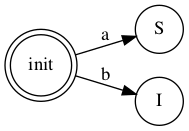
\includegraphics[width=0.25\textwidth]{agent-single-move.png}
  \caption{An open Petri-net, considering the state variable
    \texttt{init} and the enabled events that can act on ``tokens'' in
    that state variable.}
  \label{Fig:Petri1}
\end{figure}

Figre \ref{Fig:Petri1} shows an open Petri-net, focusing on the tokens
in \texttt{init}.  Each token in this case are equivalent to an aPRAM
``agent''.  In this case, the agent represented by these tokens
transitions from \texttt{init} to \texttt{S} with rate $a$, and from
\texttt{init} to \texttt{I} with rate $b$.

To translate this to an aPRAM, we take the time step for aPRAM $\delta
t$, and use the following properties.

\begin{axiom}{Markovian property:}\label{Axiom:Markov}
  Events whose rates are exponential are Markovian.  Markovian
  processes are \emph{memoryless} the next-event time for an event is
  independent of the time which has elapsed, and depends only on the
  current state of the system.
\end{axiom}

\begin{axiom}{Exponential probability distribution function:}
  The probability distribution function of an exponentially
  distributed random variable with rate $\lambda$ is given as \[f(x) =
    \lambda e^{-\lambda x}.\]  The probability distribution function
  gives the probability that the next event time is exactly $x$.
\end{axiom}

\begin{axiom}{Exponential cumulative distribution function:}
The cumulative distribution function (CDF) of an exponentially distributed
random variable with rate $\lambda$ is given as

\begin{eqnarray}
  F(x) &=& \int_{-\infty}^{x} \lambda e^{-\lambda x} dt \\
  &=& 1 - e^{-\lambda x}
\end{eqnarray}

The CDF gives the probability that the next event time is less than or
equal to $x$.
\end{axiom}

\begin{figure}
  \centering
  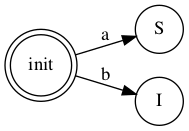
\includegraphics[width=0.25\textwidth]{agent-single-move.png}
  \caption{An open Petri-net, considering the state variable
    \texttt{init} and the enabled events that can act on ``tokens'' in
    that state variable.}
  \label{Fig:aPRAM1}
\end{figure}

In order to convert a Petri-net to an aPRAM our goal is to go from a
representation like figure \ref{Fig:Petri1}, with rates $a$ and $b$
to a representation like figure \ref{Fig:aPRAM1}, with probabilities
$x$, $y$, and $z$.  More generally, assume an agent is represented by
a token in a Petri-net.  This token can transition to other state
variables with rates given by the vector $R = [r_1, r_2, \ldots]$
which has size $|R| = n$.  The aPRAM representation of the agent this
token models is given by a vector $P = [p_0, p_1, \ldots]$ which has
size $|P| = n+1$.  We will assume $p_i$ is the probability the
transition with rate $r_i$ is chosen during an interval of length
$\delta t$, and $p_0$ is the probability the
agent does not transition during an interval of length $\delta t$.
Axiom \ref{Axiom:Markov} allows us to consider all intervals of length
$\delta t$ without concern for the elapsed simulation time.

\bibliography{references}

\end{document}